\documentclass[t,usenames,dvipsnames]{beamer}
\usetheme{Copenhagen}
\setbeamertemplate{headline}{} % remove toc from headers
\beamertemplatenavigationsymbolsempty

\usepackage{amsmath, xcolor, tikz, pgfplots, array}

\pgfplotsset{compat = newest}
\usetikzlibrary{arrows.meta, calc, decorations.pathreplacing}
\pgfplotsset{every axis/.append style = {axis lines = middle}}
\pgfplotsset{every tick label/.append style={font=\scriptsize}}
\everymath{\displaystyle}

\title{Rational Functions and Their Graphs}
\author{}
\date{}

\AtBeginSection[]
{
  \begin{frame}
    \frametitle{Objectives}
    \tableofcontents[currentsection]
  \end{frame}
}

\begin{document}

\begin{frame}
    \maketitle
\end{frame}

\begin{frame}{What is a Rational Function?}
    A \alert{rational function} is a function in the form
    \[ \frac{p(x)}{q(x)} \]
    where $p(x)$ and $q(x)$ are polynomials.
\end{frame}

\section{Determine the end behavior of a rational function}

\begin{frame}{End Behavior}
Recall from Polynomial Functions that \alert{end behavior} refers to the graph's behavior as $x$ approaches $\infty$ and also $-\infty$. \newline\\  \pause

In other words, what are the output values approaching as our input values get larger (in either direction)? 
\end{frame}

\begin{frame}{Asymptotes}
With rational functions, 1 of 2 possible scenarios for end behavior of the graph will happen with each function:    \newline\\  \pause
\begin{itemize}
    \item The function will look like a horizontal line.    \newline\\   \pause
    \item The function will not look like a horizontal line.   \newline\\ 
\end{itemize}
\end{frame}

\begin{frame}{Example 1}
Determine the end behavior of the function
\[ f(x) = \frac{2x}{x^2-3}\]   
\setlength{\extrarowheight}{3pt}
\begin{tabular}{lr}
\onslide<2->{
\begin{tabular}{c|c}
    $x$ & $f(x)$ \\ \hline
    1,000 & 0.002 \\[3pt]
    10,000 & 0.0002 \\[3pt]
    100,000 & 0.00002 \\[3pt]
    1,000,000 & 0.000002 
\end{tabular}}
&
\onslide<3->{
\begin{tabular}{c|c}
    $x$ & $f(x)$ \\ \hline
    --1,000 & --0.002 \\[3pt]
    --10,000 & --0.0002 \\[3pt]
    --100,000 & --0.00002 \\[3pt]
    --1,000,000 & --0.000002 
\end{tabular}}
\end{tabular}
\end{frame}

\begin{frame}{Example 1}
    Notice the outputs are getting closer and closer to 0. \newline\\ \pause
    
    Thus, the end behavior of the rational function
    \[ f(x) = \frac{2x}{x^2 - 3} \]
    
    is 0.   \newline\\  \pause
    
    As you zoom out of the function, the graph more and more resembles the graph of $y = 0$. \newline\\ \pause
    
    As far as notation goes, we would say
    \[ \lim_{x\to -\infty} f(x) = 0 \quad \text{and} \quad \lim_{x\to \infty} f(x) = 0 \]    
\end{frame}

\begin{frame}{End Behavior}
Determining end behavior is a result of using \alert{polynomial division}. \newline\\ \pause

When your end behavior approaches an actual number (such as 0 in the last example), then the rational function has a \alert{horizontal asymptote} as its end behavior. \newline\\ \pause

This will happen if either \newline\\
\begin{itemize}
    \item Degree of numerator $<$ Degree of denominator (horizontal asymptote will be $y = 0$)  \newline\\ \pause
    \item Degree of numerator = Degree of denominator (horizontal asymptote will be ratio of leading coefficients)
\end{itemize}
\end{frame}

\begin{frame}{Oblique Asymptotes}
If the degree of the numerator $>$ degree of the denominator, the end behavior \alert{will not be a horizontal line}. \newline\\ \pause

Instead, it will be an {\color{blue}\textbf{oblique (or slant) asymptote}}. \newline\\ \pause

You will need to use \alert{polynomial division} to find the equation of an oblique asymptote.
\end{frame}

\begin{frame}{Example 2}
Determine the end behavior of each, then find the equation of the asymptote.  \newline\\
(a) \quad $f(x) = \frac{5x}{x^2 + 1}$ \newline\\ \pause
\begin{itemize}
    \item Degree of numerator $<$ Degree of denominator \newline\\ \pause
    \item Horizontal asymptote \newline\\ \pause
    \item $y = 0$ 
\end{itemize}
\end{frame}

\begin{frame}{Example 2}
\emph{Note:} If you used polynomial division, you would get \[f(x) = {\color{red}0} + \frac{5x}{x^2+1}\]

and as $x \to \pm \infty$,  \newline\\ $f(x) \to {\color{red}0} + 0 = 0$
\end{frame}

\begin{frame}{Example 2}
(b) \quad $g(x) = \frac{x^2-4}{x+1}$ \newline\\ \pause
\begin{itemize}
    \item Degree of numerator $>$ Degree of denominator \newline\\ \pause
    \item Oblique asymptote
\end{itemize}
\end{frame}

\begin{frame}{Example 2 \quad $g(x) = \tfrac{x^2-4}{x+1}$}

\[(x^2 + 0x - 4) \div (x + 1)\] 

\begin{center}
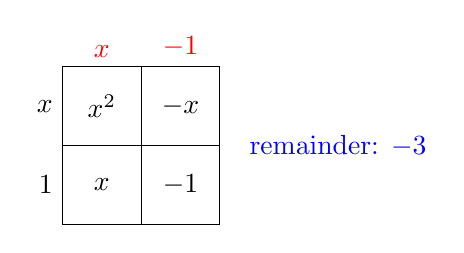
\begin{tikzpicture}
\draw (0,0) grid (2,2);
\node at (0,1.5) [left] {$x$};
\node at (0,0.5) [left] {$1$};
\node at (0.5,1.5) {$x^2$};
\onslide<2->{\node at (0.5,2) [above] {\color{red}$x$};}
\onslide<3->{\node at (0.5,0.5) {$x$};}
\onslide<4->{\node at (1.5,1.5) {$-x$};}
\onslide<5->{\node at (1.5,2) [above] {\color{red}$-1$};}
\onslide<6->{\node at (1.5,0.5) {$-1$};}
\onslide<7->{\node at (3.5,1) {\color{blue}remainder: $-3$};}
\end{tikzpicture}
\onslide<8->{\[x - 1 - \frac{3}{x+1}\]} \\[6pt]
\onslide<9->{Slant asymptote: $y = x - 1$}
\end{center}
\end{frame}

\begin{frame}{Example 2}
(c) \quad $h(x) = \frac{6x^3-3x+1}{5-2x^3}$ \pause
\[ h(x) = \frac{6x^3-3x+1}{-2x^3+5} \] \pause
\begin{itemize}
    \item Degree of numerator = Degree of denominator \newline\\ \pause
    \item Horizontal asymptote \newline\\ \pause
    \item Ratio of leading coefficients = $\tfrac{6}{-2} = -3$ \newline\\ \pause
    \item $y = -3$
\end{itemize}
\end{frame}

\begin{frame}{Example 2 \quad $h(x) = \tfrac{6x^3-3x+1}{5-2x^3}$}
\emph{Note:} If you perform polynomial division, you get
\[
h(x) = {\color{red}-3} + \frac{-3x+16}{5-2x^3}
\]

And as $x \to \pm \infty$, \newline\\
$h(x) \to {\color{red}-3} + 0 = -3$
\end{frame}


\section{Determine the equations of vertical asymptotes and coordinates of holes of a rational function}

\begin{frame}{Domain of Rational Functions}
Recall that the \alert{domain} of a rational function is all real numbers {\color{blue}\textbf{***EXCEPT***}} values that make the \alert{denominator equal 0}.   \newline\\ \pause

At each of the values that cause the denominator to = 0, there will be \textbf{only one of two things there}:  \newline\\ \pause
\begin{itemize}
    \item A vertical asymptote \newline\\ \pause
    \item Or a hole in the graph
\end{itemize}
\end{frame}

\begin{frame}{Vertical Asymptotes}
A \alert{vertical asymptote} is a vertical line that the function will approach, but \underline{never intersect}.    \newline\\ \pause

As the graph of the function gets closer to a vertical asymptote, the graph will either skyrocket up towards $\infty$ or plummet downward towards $-\infty$. 
\end{frame}

\begin{frame}{Vertical Asymptotes}
\begin{center}
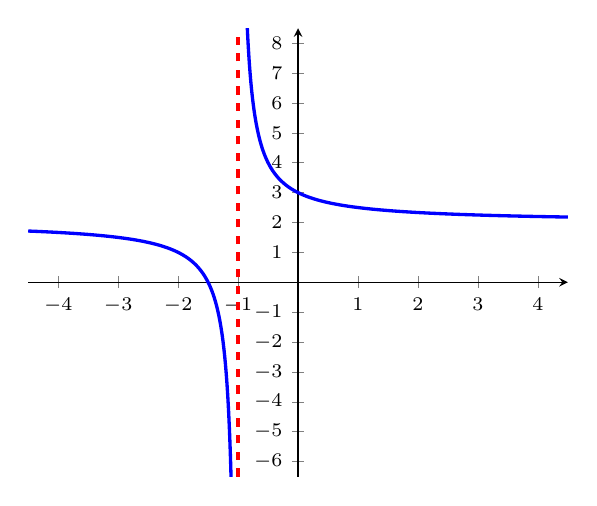
\begin{tikzpicture}
\begin{axis}[
xmin = -4.5, xmax = 4.5,
ymin = -6.5, ymax = 8.5,
xtick = {-4,-3,...,4},
ytick = {-6,-5,...,8}
]
\addplot[color=blue, very thick, samples=200, smooth, domain=-4.5:-1.05] {(1/(x+1) + 2};
\addplot[color=blue, very thick, samples=200, smooth, domain=-0.95:4.5] {(1/(x+1) + 2};
\draw[red, dashed, very thick] (axis cs: -1,-6.5) -- (axis cs: -1,8.5);
\end{axis}
\end{tikzpicture}
\end{center}
\end{frame}

\begin{frame}{Holes in Rational Functions}
Most graphing technology will not show holes in graphs upon sight.
\end{frame}

\begin{frame}{How to Tell Your Asymptote From a Hole In the Graph}
    \begin{enumerate}
        \item \alert{Factor} both numerator and denominator \textbf{**completely**} and then {\color{blue}\textbf{simplify that}}. \newline\\ \pause
        \item For {\color{violet}\textbf{each domain issue}} in the \underline{denominator}: \newline\\ \pause
        \begin{itemize}
            \item If you get a 0 in the denominator after evaluating the simplified expression, you have a \alert{vertical asymptote}.  \newline\\ \pause
            \item Otherwise, there is a hole in the graph there.    \newline\\ \pause
        \end{itemize}
    \end{enumerate}
To get the $y$-coordinate of a hole in the graph, plug in the value of $x$ into your simplified expression.
\end{frame}

\begin{frame}{Example 3}
Determine the domain of each. Then determine the equations of vertical asymptotes and/or coordinates of any holes.  \newline\\
(a) \quad $f(x) = \frac{2x}{x^2-9}$ 
\onslide<2->{$= \frac{2x}{(x+3)(x-3)}$} \newline\\
\onslide<3->{Domain:}
\begin{align*}
    \onslide<4->{x+3 &\neq 0 & x-3&\neq 0} \\
    \onslide<5->{x &\neq -3 & x&\neq 3} \\
\end{align*}
\onslide<6->{Domain: $x \neq -3, 3$}
\end{frame}

\begin{frame}{Example 3 \quad Domain: $x\neq-3, 3$}
\[ f(x) = \frac{2x}{(x+3)(x-3)} \] 
\onslide<2->{We get 0s in denominator if we evaluate \[\frac{2x}{(x+3)(x-3)}\] at $x = -3\text{ and } x=3$} \newline\\
\onslide<3->{$x = -3$ and $x = 3$ are both {\color{red}vertical asymptotes}} \newline\\
\onslide<4->{There are no holes in the graph}
\end{frame}

\begin{frame}{Example 3}
(b) \quad $g(x) = \frac{x^2-6x-7}{x^2+5x+4}$
\onslide<2->{$=\frac{(x+1)(x-7)}{(x+1)(x+4)}$ \onslide<5->{$=\frac{x-7}{x+4}$}} \\[15pt]
\onslide<3->{Domain: }
\onslide<4->{$x \neq -4,-1$} \newline\\
\onslide<6->{Vertical asymptote at $x=-4$} \newline\\
\onslide<7->{Hole in graph at $x = -1$} 
\onslide<8->{\[\text{$y$-coordinate: } \frac{-1-7}{-1+4} = -\frac{8}{3}\]}
\onslide<9->{Hole at $\left(-1, -\frac{8}{3}\right)$}
\end{frame}

\begin{frame}{Example 3}
(c) \quad $h(x) = \frac{x^2-x-6}{x^2-9}$
\onslide<2->{$= \frac{(x-3)(x+2)}{(x-3)(x+3)}$ \onslide<5->{$=\frac{x+2}{x+3}$}} \\[15pt]
\onslide<3->{Domain: } 
\onslide<4->{$x \neq -3,3$} \newline\\
\onslide<6->{Vertical asymptote at $x=-3$} \newline\\
\onslide<7->{There is a hole in the graph at $x=3$}
\onslide<8->{\[\text{$y$-coordinate: } \frac{3+2}{3+3} = \frac{5}{6}\]}
\onslide<9->{Hole at $\left(3, \frac{5}{6}\right)$}
\end{frame}

\begin{frame}{Example 3}
(d) \quad $j(x) = \frac{x^2-x-6}{x^2+9}$
\onslide<2->{$=\frac{(x-3)(x+2)}{x^2+9}$} \\[15pt]
\onslide<3->{Since $x^2+9\neq 0$ for any real number $x$, domain is All Real Numbers} \\[15pt]
\onslide<4->{Since domain is all reals, there are no vertical asymptotes or holes}
\end{frame}

\begin{frame}{Example 3}
(e) \quad $k(x) = \frac{x^2-x-6}{x^2+4x+4}$
\onslide<2->{$=\frac{(x-3)(x+2)}{(x+2)(x+2)}$}
\onslide<5->{$=\frac{x-3}{x+2}$} \\[15pt]
\onslide<3->{Domain: }
\onslide<4->{$x \neq -2$} \newline\\
\onslide<6->{Vertical asymptote at $x=-2$} \newline\\
\onslide<7->{There is no hole in the graph}
\end{frame}

\end{document}
